% Options for packages loaded elsewhere
\PassOptionsToPackage{unicode}{hyperref}
\PassOptionsToPackage{hyphens}{url}
%
\documentclass[
]{article}
\usepackage{amsmath,amssymb}
\usepackage{lmodern}
\usepackage{iftex}
\ifPDFTeX
  \usepackage[T1]{fontenc}
  \usepackage[utf8]{inputenc}
  \usepackage{textcomp} % provide euro and other symbols
\else % if luatex or xetex
  \usepackage{unicode-math}
  \defaultfontfeatures{Scale=MatchLowercase}
  \defaultfontfeatures[\rmfamily]{Ligatures=TeX,Scale=1}
\fi
% Use upquote if available, for straight quotes in verbatim environments
\IfFileExists{upquote.sty}{\usepackage{upquote}}{}
\IfFileExists{microtype.sty}{% use microtype if available
  \usepackage[]{microtype}
  \UseMicrotypeSet[protrusion]{basicmath} % disable protrusion for tt fonts
}{}
\makeatletter
\@ifundefined{KOMAClassName}{% if non-KOMA class
  \IfFileExists{parskip.sty}{%
    \usepackage{parskip}
  }{% else
    \setlength{\parindent}{0pt}
    \setlength{\parskip}{6pt plus 2pt minus 1pt}}
}{% if KOMA class
  \KOMAoptions{parskip=half}}
\makeatother
\usepackage{xcolor}
\IfFileExists{xurl.sty}{\usepackage{xurl}}{} % add URL line breaks if available
\IfFileExists{bookmark.sty}{\usepackage{bookmark}}{\usepackage{hyperref}}
\hypersetup{
  hidelinks,
  pdfcreator={LaTeX via pandoc}}
\urlstyle{same} % disable monospaced font for URLs
\usepackage{color}
\usepackage{fancyvrb}
\newcommand{\VerbBar}{|}
\newcommand{\VERB}{\Verb[commandchars=\\\{\}]}
\DefineVerbatimEnvironment{Highlighting}{Verbatim}{commandchars=\\\{\}}
% Add ',fontsize=\small' for more characters per line
\newenvironment{Shaded}{}{}
\newcommand{\AlertTok}[1]{\textcolor[rgb]{1.00,0.00,0.00}{\textbf{#1}}}
\newcommand{\AnnotationTok}[1]{\textcolor[rgb]{0.38,0.63,0.69}{\textbf{\textit{#1}}}}
\newcommand{\AttributeTok}[1]{\textcolor[rgb]{0.49,0.56,0.16}{#1}}
\newcommand{\BaseNTok}[1]{\textcolor[rgb]{0.25,0.63,0.44}{#1}}
\newcommand{\BuiltInTok}[1]{#1}
\newcommand{\CharTok}[1]{\textcolor[rgb]{0.25,0.44,0.63}{#1}}
\newcommand{\CommentTok}[1]{\textcolor[rgb]{0.38,0.63,0.69}{\textit{#1}}}
\newcommand{\CommentVarTok}[1]{\textcolor[rgb]{0.38,0.63,0.69}{\textbf{\textit{#1}}}}
\newcommand{\ConstantTok}[1]{\textcolor[rgb]{0.53,0.00,0.00}{#1}}
\newcommand{\ControlFlowTok}[1]{\textcolor[rgb]{0.00,0.44,0.13}{\textbf{#1}}}
\newcommand{\DataTypeTok}[1]{\textcolor[rgb]{0.56,0.13,0.00}{#1}}
\newcommand{\DecValTok}[1]{\textcolor[rgb]{0.25,0.63,0.44}{#1}}
\newcommand{\DocumentationTok}[1]{\textcolor[rgb]{0.73,0.13,0.13}{\textit{#1}}}
\newcommand{\ErrorTok}[1]{\textcolor[rgb]{1.00,0.00,0.00}{\textbf{#1}}}
\newcommand{\ExtensionTok}[1]{#1}
\newcommand{\FloatTok}[1]{\textcolor[rgb]{0.25,0.63,0.44}{#1}}
\newcommand{\FunctionTok}[1]{\textcolor[rgb]{0.02,0.16,0.49}{#1}}
\newcommand{\ImportTok}[1]{#1}
\newcommand{\InformationTok}[1]{\textcolor[rgb]{0.38,0.63,0.69}{\textbf{\textit{#1}}}}
\newcommand{\KeywordTok}[1]{\textcolor[rgb]{0.00,0.44,0.13}{\textbf{#1}}}
\newcommand{\NormalTok}[1]{#1}
\newcommand{\OperatorTok}[1]{\textcolor[rgb]{0.40,0.40,0.40}{#1}}
\newcommand{\OtherTok}[1]{\textcolor[rgb]{0.00,0.44,0.13}{#1}}
\newcommand{\PreprocessorTok}[1]{\textcolor[rgb]{0.74,0.48,0.00}{#1}}
\newcommand{\RegionMarkerTok}[1]{#1}
\newcommand{\SpecialCharTok}[1]{\textcolor[rgb]{0.25,0.44,0.63}{#1}}
\newcommand{\SpecialStringTok}[1]{\textcolor[rgb]{0.73,0.40,0.53}{#1}}
\newcommand{\StringTok}[1]{\textcolor[rgb]{0.25,0.44,0.63}{#1}}
\newcommand{\VariableTok}[1]{\textcolor[rgb]{0.10,0.09,0.49}{#1}}
\newcommand{\VerbatimStringTok}[1]{\textcolor[rgb]{0.25,0.44,0.63}{#1}}
\newcommand{\WarningTok}[1]{\textcolor[rgb]{0.38,0.63,0.69}{\textbf{\textit{#1}}}}
\usepackage{graphicx}
\makeatletter
\def\maxwidth{\ifdim\Gin@nat@width>\linewidth\linewidth\else\Gin@nat@width\fi}
\def\maxheight{\ifdim\Gin@nat@height>\textheight\textheight\else\Gin@nat@height\fi}
\makeatother
% Scale images if necessary, so that they will not overflow the page
% margins by default, and it is still possible to overwrite the defaults
% using explicit options in \includegraphics[width, height, ...]{}
\setkeys{Gin}{width=\maxwidth,height=\maxheight,keepaspectratio}
% Set default figure placement to htbp
\makeatletter
\def\fps@figure{htbp}
\makeatother
\usepackage[normalem]{ulem}
% Avoid problems with \sout in headers with hyperref
\pdfstringdefDisableCommands{\renewcommand{\sout}{}}
\setlength{\emergencystretch}{3em} % prevent overfull lines
\providecommand{\tightlist}{%
  \setlength{\itemsep}{0pt}\setlength{\parskip}{0pt}}
\setcounter{secnumdepth}{-\maxdimen} % remove section numbering
\ifLuaTeX
  \usepackage{selnolig}  % disable illegal ligatures
\fi

\author{}
\date{}

\begin{document}

\hypertarget{pandoc-image-sizing-when-converting-from-jupyter-notebook-to-latex}{%
\subsection{Pandoc image sizing when converting from Jupyter notebook to
LaTeX}\label{pandoc-image-sizing-when-converting-from-jupyter-notebook-to-latex}}

I am attempting to use \texttt{pandoc} to convert a Jupyter Notebook
into a readable pdf. I have read the
\href{https://pandoc.org/MANUAL.html\#images}{pandoc manual} section
regarding images. \sout{Unfortunately the \mbox{\texttt{ipynb}} to
\mbox{\texttt{pdf}} does not appear to be working as expected.}

\begin{Shaded}
\begin{Highlighting}[]
\ExtensionTok{pandoc} \AttributeTok{{-}{-}version}
\end{Highlighting}
\end{Shaded}

gives

\begin{verbatim}
pandoc 2.12
Compiled with pandoc-types 1.22, texmath 0.12.1.1, skylighting 0.10.4,
citeproc 0.3.0.8, ipynb 0.1.0.1
\end{verbatim}

Here is an image, where I would like to specify the width

\begin{figure}
\centering
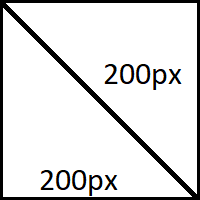
\includegraphics[width=1cm,height=\textheight]{test_image.png}
\caption{Image Caption}
\end{figure}

\begin{Shaded}
\begin{Highlighting}[]
\AlertTok{![Image Caption](test\_image.png)}\NormalTok{\{ width=1cm \}}
\end{Highlighting}
\end{Shaded}

Running:

\begin{Shaded}
\begin{Highlighting}[]
\ExtensionTok{pandoc} \AttributeTok{{-}s} \AttributeTok{{-}o}\NormalTok{ README.tex README.md}
\ExtensionTok{xelatex}\NormalTok{ README.tex}
\end{Highlighting}
\end{Shaded}

gives:

\begin{Shaded}
\begin{Highlighting}[]
\KeywordTok{\textbackslash{}begin}\NormalTok{\{}\ExtensionTok{figure}\NormalTok{\}}
\FunctionTok{\textbackslash{}centering}
\BuiltInTok{\textbackslash{}includegraphics}\NormalTok{[width=1cm,height=}\FunctionTok{\textbackslash{}textheight}\NormalTok{]\{}\ExtensionTok{test\_image.png}\NormalTok{\}}
\FunctionTok{\textbackslash{}caption}\NormalTok{\{Image Caption\}}
\KeywordTok{\textbackslash{}end}\NormalTok{\{}\ExtensionTok{figure}\NormalTok{\}}
\end{Highlighting}
\end{Shaded}

And, if I put

\begin{Shaded}
\begin{Highlighting}[]
\AlertTok{![Image Caption](test\_image.png)}\NormalTok{\{ width=1cm \}}
\end{Highlighting}
\end{Shaded}

in a markdown cell in a notebook, and run

\begin{Shaded}
\begin{Highlighting}[]
\ExtensionTok{pandoc} \AttributeTok{{-}{-}from}\NormalTok{ ipynb+link\_attributes }\AttributeTok{{-}s} \AttributeTok{{-}o}\NormalTok{ Pandoc\_problems.tex Pandoc\_problems.ipynb}
\ExtensionTok{xelatex}\NormalTok{ Pandoc\_problems.tex}
\end{Highlighting}
\end{Shaded}

I get:

\begin{Shaded}
\begin{Highlighting}[]
\BuiltInTok{\textbackslash{}includegraphics}\NormalTok{[width=1cm,height=}\FunctionTok{\textbackslash{}textheight}\NormalTok{]\{}\ExtensionTok{test\_image.png}\NormalTok{\}}
\end{Highlighting}
\end{Shaded}


\end{document}
